%%%%%%%%%%%%%%%%%%%%%%%%%%%%%%%%%%%%%%%%%
% Original author:
% Linux and Unix Users Group at Virginia Tech Wiki
% (https://vtluug.org/wiki/Example_LaTeX_chem_lab_report)
% Modified by: Hector F. Jimenez S, for the Digital Electronics Laboratory.
% License:
% CC BY-NC-SA 3.0 
%%%%%%%%%%%%%%%%%%%%%%%%%%%%%%%%%%%%%%%%%
%----------------------------------------
%	PACKAGES AND DOCUMENT CONFIGURATIONS
%---------------------------------------

\documentclass[paper=a4, fontsize=12pt]{article} 		% A4 paper and 11pt font size
\usepackage[T1]{fontenc} 								% Use 8-bit encoding that has 256 glyphs
%\usepackage{fourier}		 							% Use the Adobe Utopia font for the document 
\usepackage[spanish,english]{babel}						% Spanish Language, templates uses some sections in english.
\selectlanguage{spanish}								% main language.
\PassOptionsToPackage{spanish}{babel}
%\renewcommand{\figurename}{Figura}						% Force rename of figure.
%\renewcommand{\figurename}{Fig.}
\usepackage[figurename=Fig.]{caption}
\usepackage[utf8]{inputenc}								% tildes for spanish language.
\usepackage{amsmath,amsfonts,amsthm} 					% Math packages.
\usepackage{minted}										% For syntax highlighting.
\usepackage{float}										% Image will be in the same place as you want.!!! x-/
\usepackage{sectsty} 									% Allows customizing section commands
\allsectionsfont{\centering \normalfont\scshape}	   	% Make all sections centered, the default font and small caps
\usepackage{hyperref}
\hypersetup{											%Setups the false color and borders.
    colorlinks=false,
    pdfborder={0 0 0},
}
\newcommand\fnurl[2]{%									% set a simple and quick footnote command and include url.
\href{#2}{#1}\footnote{\url{#2}}%	
}
\usepackage{graphicx}									% Import easyly images.
\graphicspath{ {./images/} }							% Where to look for the images.
\DeclareGraphicsExtensions{.pdf,.png,.jpg}				% Graphics Extension to be used
\usepackage[notes,backend=biber]{biblatex-chicago}		% Bibliography and references.
\bibliography{biblio}									% bibliography filename.
\usepackage{fancyhdr} 									% Custom headers and footers
\pagestyle{fancyplain} 									% Makes all pages in the document conform to the custom headers and footers
\fancyhead{} 											% No page header
\fancyfoot[L]{} 										% Empty left footer
\fancyfoot[C]{} 										% Empty center footer
\fancyfoot[R]{\thepage} 								% Page numbering for right footer
\renewcommand{\headrulewidth}{0pt} 						% Remove header underlines
\renewcommand{\footrulewidth}{0pt} 						% Remove footer underlines
\setlength{\headheight}{13.6pt} 					    % Customize the height of the header
\numberwithin{equation}{section}						% Number equations within sections (i.e. 1.1, 1.2, 2.1, 2.2 instead of 1, 2, 3, 4)
%\numberwithin{figure}{section} 						% Number figures within sections (i.e. 1.1, 1.2, 2.1, 2.2 instead of 1, 2)
\numberwithin{table}{section} 							% Number tables within sections (i.e. 1.1, 1.2, 2.1, 2.2 instead of 1, 2, 3, 4)
\setlength\parindent{0pt} 								% Removes all indentation from paragraphs

%\newcommand{\horrule}[1]{\rule{\linewidth}{#1}} 		% Create horizontal rule command with 1 argument of height
%%%%%%%%%%%%%%%%%%%%
%Title Section
%%%%%%%%%%%%%%%%%%%%%
\title{Desarrollo de un Controlador de Tráfico\\ 
Usando FPGA's \\
Laboratorio de Electrónica Digital\\Módulo: 1} 			% Title
%\horrule{0.5pt} \\[0.4cm] 								% Thin top horizontal rule	Title rule
%\huge Assignment Title \\ 								% The assignment title
%\horrule{2pt} \\[0.5cm] 								% Thick bottom horizontal rule
\author{												% Authors begin.
Héctor F. \textsc{Jiménez Saldarriaga}\\
\texttt{hfjimenez@utp.edu.co} \\
\texttt{PGP KEY ID: 0xB05AD7B8}
\and
Steffany \textsc{Lopez Segura}\\
\texttt{steffany@utp.edu.co}
} 												       % End of  Author name
\date{}    						                       % Date for the report, this will hide the \today.

\begin{document}
\maketitle                      			           % Insert the title, author and date
\begin{center}
\begin{tabular}{l r}								   % two column to
Fecha de Entrega: & Febrero 24, 2016 \\				   % Ramiro's Details.
Profesor: & Ing.Msc(c) Ramiro Andres Barrios Valencia
\end{tabular}
\end{center}
%%%%%%%%%%%	
% Let's start the document.
%%%%%%%%%%%	
\section{Objectivos}
\begin{itemize}
  \item Fortalecer y poner en práctica la teoría de circuitos combinacionales.
  \item Fortalecer el desarrollo de sistemas digitales, utilizando el lenguaje \emph{VHDL} y el entorno de desarrollo Xilinx ISE.
  \item Identificar la arquitectura, esquemáticos y hardware integrado de la placa de desarrollo \emph{NEXYS2}.
  \item Implementar en lenguaje VHDL un módulo que permita la detección correcta de los pulsos entregados por los botones presentes en la tarjeta de desarrollo\footnote{Datasheet Oficial de la placa  Nexys 2 \fnurl{Manual}{http://reference.digilentinc.com/_media/nexys:nexys2:nexys2_rm.pdf}}
  \item Identificar posibles problemas a la hora de acoplar los otros módulos a desarrollar.
\end{itemize}

%%%%%%%%%%%	
% Theory Marc! 
%%%%%%%%%%%	
\section{Marco Teórico}
\label{sec:problemamecanico}
Utilizar switches y pulsadores mecánicos en un sistema electrónico es una práctica muy común, pues sirven de interface entre el usuario y el sistema embebido para seleccionar y programar funciones que este posee; en la práctica actual muchos de estos sistemas mecánicos están siendo reemplazados por displays táctiles pero hay situaciones industriales principalmente en las cuales un pulsador mecánico sería una solución más apropiada y eficiente en la implementación, pues al ser un sistemas mecánicos estos no se degradan tan rápido como lo harían las pantallas táctiles en un entorno industrial. Una de las grandes desventajas que poseen los pulsadores son los rebotes o saltos como se puede observar en la figura \ref{fig:debounce}.\\
\begin{figure}[H]
  \centering
     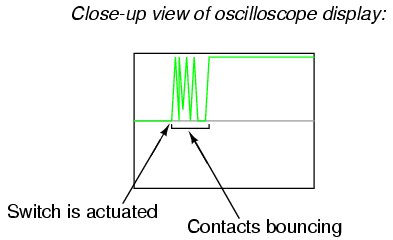
\includegraphics[width=0.7\textwidth]{debounce}
  \caption{Rebotes al presionar un pulsador mecánico, señales de osciloscopio.}
      \label{fig:debounce}
\end{figure}
Los elementos mecánicos del pulsador están constituidos por un par de contactos eléctricos que se unen o separan por medios mecánicos,  en la figura \ref{fig:pulsador} se muestra un pulsador común, figuras\ref{fig:pulsadorinternal1} \ref{fig:pulsadorinternal2} son vista detalladas. Los falsos contactos que se producen cuando los accionamos, crean falsas señales instantáneas, ocasionando un mal funcionamiento del dispositivo, no olvidando mencionar que existe una barrera o GAP que se produce por el aire entre los elementos mecanicos\textit{( aunque típicamente esto es despreciable por su baja fuerza discipativa)} induciendo múltiples pulsaciones o flancos como se muestra en la figura \ref{fig:debounce}. 
\begin{figure}[H]
  \centering
     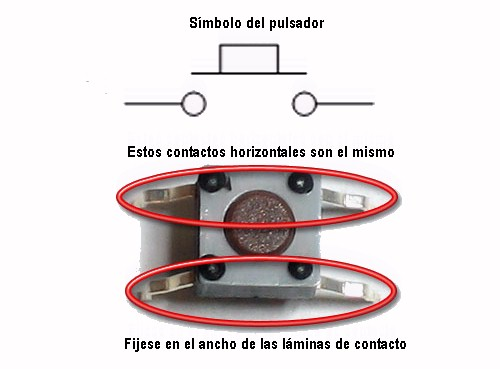
\includegraphics[width=0.5\textwidth]{pulsador}
  \caption{Pulsador Común, Composición.}
      \label{fig:pulsador}
\end{figure}

\begin{figure}[H]
  \centering
     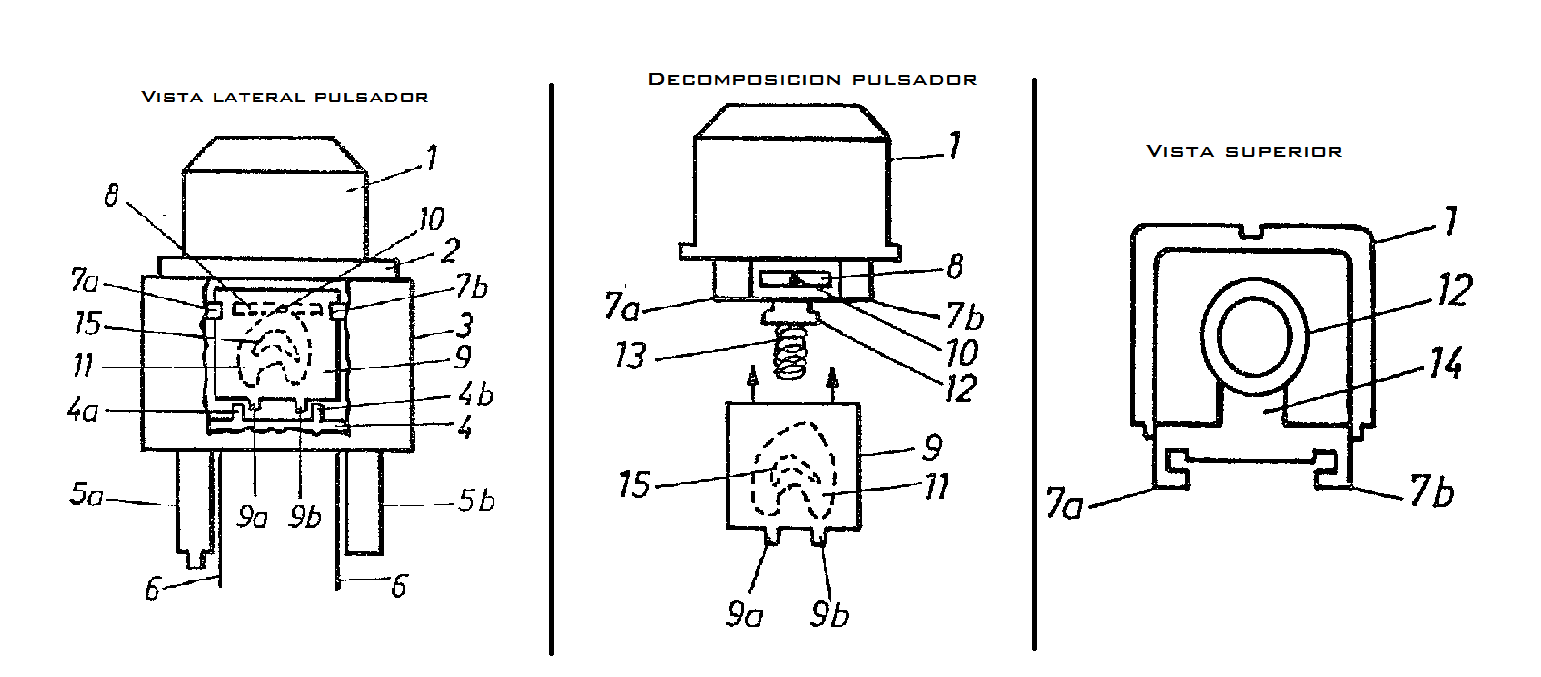
\includegraphics[width=0.7\textwidth]{pulsadorinternals}
  \caption{Decomposicion de un Pulsador común}
      \label{fig:pulsadorinternal1}
\end{figure}
\begin{figure}[H]
  \centering
     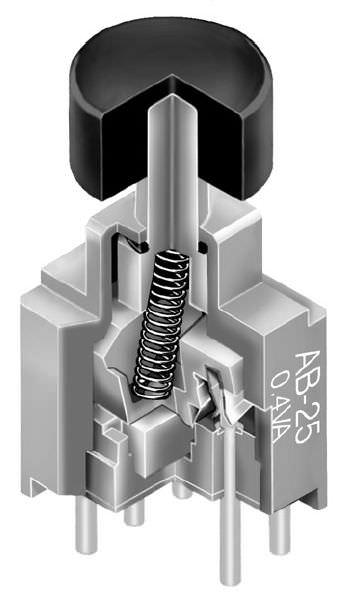
\includegraphics[width=0.2\textwidth]{internal}
  \caption{Vista en 3d de un pulsador y sus elementos }
      \label{fig:pulsadorinternal2}
\end{figure}
\label{sec:pulsador} 
En algunos casos esta acción puede producir una chispa debido a la corriente que atraviesa los contactos, disminuyendo el tiempo útil de los contactos eléctricos. La chispa se produce siempre al separar los contactos (desconectar), en ocasiones parece que también salta al conectarlos, eso es debido a los rebotes mecánicos que se producen al cambiar de estado.
Existen muchas formas de lidiar con este problema, tanto soluciones por hardware físico como el circuito simple de la figura \ref{fig:hardwc} o por software como lo realizaremos para el desarrollo de este modulo, mediante la implementación de un circuito lógico provisto por la empresa \fnurl{Digikey.}{http://www.digikey.com/}\\
\begin{figure}[H]
  \centering
     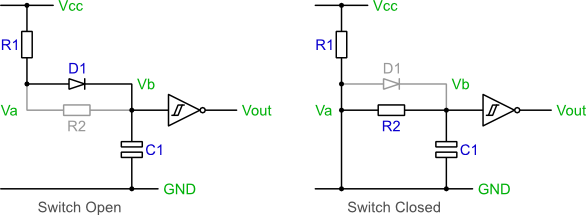
\includegraphics[width=0.7\textwidth]{debounceCircuit2}
  \caption{Solución utilizando un simple arreglo electrónico. Pulsadores con resistencias de Pull Ups.}
      \label{fig:hardwc}
\end{figure}
\section{Arquitectura de la Placa \emph{NEXYS 2}}
La tarjeta de entrenamiento \emph{NEXYS 2} es una plataforma de desarrollo fabricada por la empresa \footnote{Digilentinc Página Oficial \fnurl{Nexys2 Spartan3E}{http://store.digilentinc.com/nexys-2-spartan-3e-fpga-trainer-board-retired-see-nexys-4-ddr/}} aunque se encuentra descontinuada para la venta y recomiendan utilizar esta misma en su version \textbf{4}, utiliza una fpga Spartan 3E optimizada para desarrollo de aplicaciones donde se requiere implementar diseños de lógica compleja, e ideal para el procesamiento de señales y desarrollo de sistemas embebidos como se menciona en \fnurl{General Spartan Versions}{http://www.xilinx.com/support/documentation-navigation/silicon-devices/mature-products/spartan-3e.html}, \fnurl{Spartan-3E FPGA Family: Introduction and Ordering Information}{http://www.xilinx.com/support/documentation/data_sheets/ds312.pdf}.
\\Algunos elementos destacables de la placa son :
\begin{description}
  \item[Connectores] \hfill \\
  	\begin{itemize}
		\item Puerto USB2.0
	    \item Puerto VGA
		\item PS/2
	    \item Puerto RS232
    \end{itemize}
\begin{figure}[H]
 \centering
   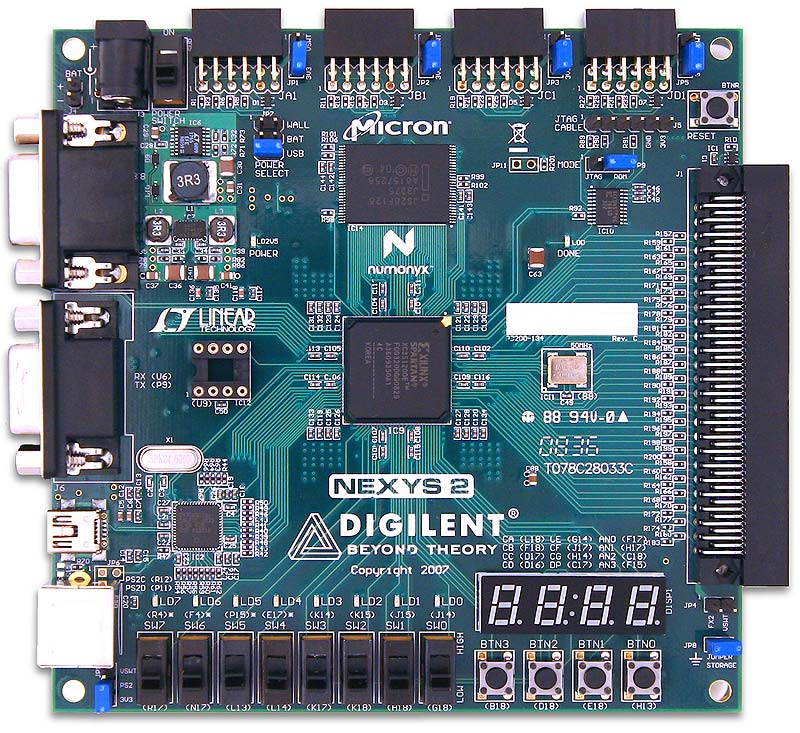
\includegraphics[width=0.7\textwidth]{model}
 \caption{Modelo de la Nexxys , Versión 2.}
    \label{fig:modelo}
\end{figure}
Algunas de las que más nos llamaron la atención son:\\
  \item[Caracteristicas] \hfill \\
    	\begin{itemize}
			\item Xilinx Spartan-3E FPGA 500K
			\item Memoria PSDRAM de 16 MB fast Micron® 
			\item Memoria de 16 MB Intel® StrataFlash® Flash R 
      		\item Trabaja con la version Free de ISE®/WebPACK 
            \item Oscillador de 50 MHz
			\item Fuentes reguladas de 3.3V@3A/100mA(principal),3.3V@150mA/60mA,2.5V/1.2V@1.4A/50mA
            \item Todas las entradas tiene protección contra cortocircuitos y descargas electroestática
  			\item Incluye  8 leds, cuatro display siete segmentos, cuatro pulsadores, 8 switches.\ldots
      \end{itemize}
\end{description}
Para plantear una solución al problema mencionado en \ref{sec:problemamecanico}, nosotros hemos descargado el esquemático para comprender circuitalmente cuál es la configuración de los pulsadores, aunque generalmente para desarrollos importantes en electrónica, se compran  pulsadores de alta calidad, y resistencia mecánica a presiones momentáneas e instantáneas, pero dado que esto es una placa de entrenamiento, \textit{estudiantil} asumimos que los pulsadores que esta posee son netamente mecánicos que cuenta con el diseño de la figura \ref{fig:btn}
\begin{figure}[H]
  \centering
     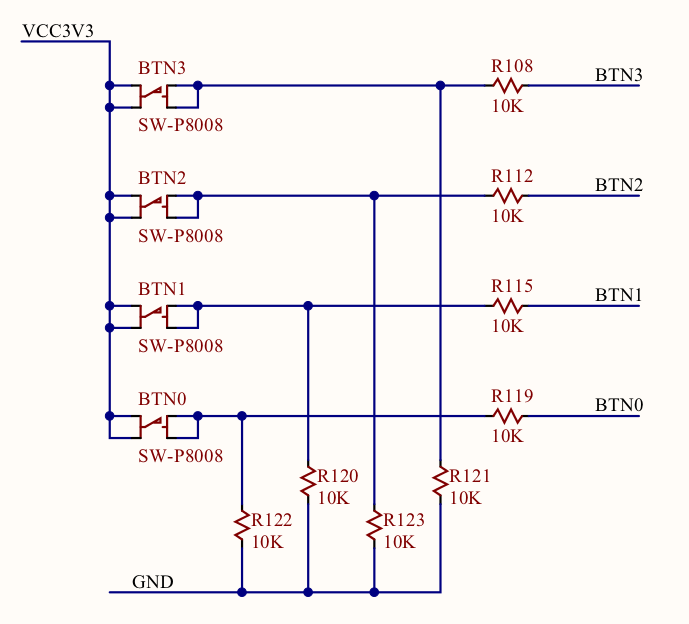
\includegraphics[width=0.5\textwidth]{btn1.png}
  \caption{Esquema provisto en el esquemático, 4 pulsadores.}
    \label{fig:btn}
\end{figure}

\begin{figure}[H]
  \centering
     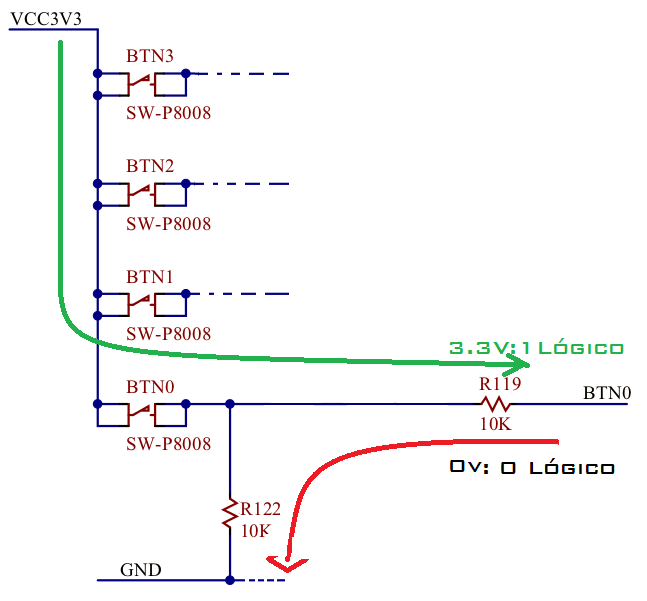
\includegraphics[width=0.6\textwidth]{btn2.png}
  \caption{Circulación de la corriente en el circuito, resistencia de 10k$\Omega$ protección contra cortocircuito}
      \label{fig:btn2}
\end{figure}
La figura \ref{fig:btn2} también muestra una configuración de un solo pulsador vemos la resistencia de pull down. Con colores hemos indicado el accionamiento del pulsador, tome como ejemplo \ref{fig:btn2}, el color rojo indica cuando el pulsador \textbf{BTN0} no ha sido presionado, esto indica que los pulsadores son de tipo \textbf{N.O} ó \textit{Normally Open in Low Mode} presentando un \textbf{0 lógico} a la salida, al presionar el pulsador, el contacto interno que este posee cierra el circuito conectándolo con la fuente de 3.3v como lo muestra el color verde de la figura \ref{fig:btn2}.

\section{Antirebote por Software}
Resolver el problema de los rebotes de un pulsador puede ser una tarea fácil o compleja, la idea básica es \emph{muestrear} la señales de entrada de los pulsadores en un intervalo regular de tiempo para notar si hay cambios en la entrada, si no existieron cambios se debe mantener el estado actual del pulsador, si hay pulsos anormales debemos filtrar la señal. Hay dos aproximaciones como se menciona en el sitio web \fnurl{Labbookpages.co.uk}{http://www.labbookpages.co.uk/electronics/debounce.html} para un configuración de pull up, nosotros utilizaremos esto mismo para una configuración de pull-down sin decidir si será modulo ya que debemos realizar prácticas experimentales con la tarjeta:
\begin{itemize}
	\item[Contador] Este contador  nos dirá cuanto tiempo ha pasado desde que la señal ha estado en alto, si la señal  ha estado en alto durante un tiempo definido por nosotros \textit{(50 mS)}, entonces es considerado como un pulso estable, y debería de setear la salida a 1. Esta aproximación es parecida vista en la implementación de \fnurl{DigiKey}{https://eewiki.net/pages/viewpage.action?pageId=4980758} pero más completa.
    \item[Registro 8bits] Esta aproximación es similar a la mencionada anteriormente, pero utiliza un registro de desplazamiento de 8bits en vez de un contador, lo que hace es ir desplazando los bits hasta alcanzar su valor máximo.

\end{itemize}

\begin{figure}[H]
  \centering
     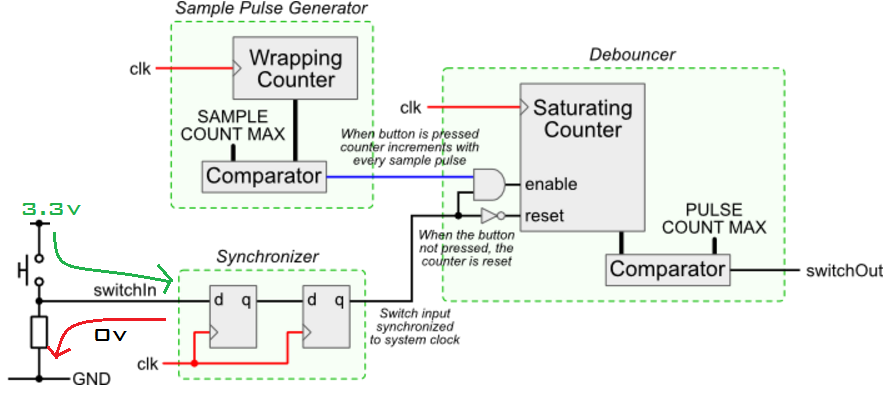
\includegraphics[width=1\textwidth]{implementacion}
  \caption{Desarrollo a implementar. Tiempo para presionar el pulsador mínimo de 33mS}
  \label{fig:eliteimplemetacion}
\end{figure}
La figura \ref{fig:eliteimplemetacion} está compuesta por tres partes principales donde cada una tiene encargada una función como se muestra  a continuación\\
\newline
\textbf{Sample Pulse Generator}: Es un contador que incrementa el reloj en cada cambio de flanco Cuando el alcanza la máxima cantidad de pulsos muestreados un pulso es generado y la cuenta se reinicia, el pulso muestreado es usado para muestrear la entrada del pulsador.\\
\newline
\textbf{Synchroniser}: Se encarga de sincronizar la señal de entrada en la figura \ref{fig:eliteimplemetacion} \textbf{SwitchIn} con la señal de reloj, así que si no se presiona el pulsador el contador estará deshabilitado, ya que su reset es activo bajo.\\
\newline
\textbf{Debouncer}: Este contador se incrementa en cada pulso muestreado cuando el pulsador es presionado. Cuando el pulsador no es presionado el contador está en reset. Si el contador llega a su valor máximo, la salida del comparador se pone en alto, de lo contrario está en bajo.
\textbf{AGREGAR ECUACIONES DE TIEMPOS!}
\newline
\section{Explicación Código VHDL}
Descripción del Pseudo código para el módulo anti rebote:
\begin{minted}{vhdl}
 1 Setup a counter variable, initialise to zero.
 2 Setup a regular sampling event, perhaps using a timer. Use a period of about 1ms.
 3 On a sample event:
 4   if switch signal is high then
 5     Reset the counter varaible to zero
 6     Set internal switch state to released
 7   else
 8     Increment the counter variable to a maximum of 10
 9   end if
10   if counter=10 then
11     Set internal switch state to pressed
12   end if
\end{minted}
Código de Ejemplo de Anti-Rebote.
%\inputminted{vhdl}{./Code/debounce.vhd}
\section{Prácticas Experimentales}
Fotos de la Simulación y Conclusiones.
\section{Anexos}
Se adjunta el código en un archivo comprimido de nombre \textsc{module1.zip}, los demás archivos son adicionales que resuelven la misma implementación.
\textit{Nota}: Las referencias utilizadas se encuentran en los pies de página. Si requiere de manera detallada estas contacte con \emph{hfjimenez@utp.edu.co}
\end{document}